3%*******10********20********30********40********50********60********70********80

% For all chapters, use the newdefined chap{} instead of chapter{}
% This will make the text at the top-left of the page be the same as the chapter

\chap{Σχεδιασμός \& Υλοποίηση Εφαρμογής} \label{c:crypto}



Στο κεφάλαιο 2, διερευνήσαμε το πεδίο της επαυξημένης πραγματικότητας και τις μαθηματικές αρχές από τις οποίες διέπεται. Παρουσιάσαμε επίσης τη χρησιμότητα της ενσωμάτωσης δυνατοτήτων αναγνώρισης χειρονομιών σε εφαρμογές, καθώς και ερευνητικές εργασίες σχετικές με τη διπλωματική αυτή εργασία. 
Όπως αναφέρθηκε, πολλές εφαρμογές επαυξημένης πραγματικότητας έχουν αναπτυχθεί στον τομέα των βιντεοπαιχνιδιών. 

The suitable architecture and frameworks presented previously, chapter 3 are implemented in this section, starting with a summary of the development tools and equipment required. At first, we show the implementation of the basic scenario in the Unity engine, after we present the
description of the evaluation performed with two tasks and the experimental set-up used.



Στις παρακάτω ενότητες θα πραγματοποιηθεί ανάλυση των μεθόδων που αναπτύχθηκαν για την δημιουργία ενός σκακιού επαυξημένης πραγματικότητας, όπου ο χρήστης μπορεί να χειριστεί εικονικά πιόνια μόνο με τα χέρια του με χειρονομίες "τσιμπήματος". Αρχικά θα παρουσιαστούν τα εργαλεία και ο αισθητήρας που χρησιμοποιήθηκαν, καθώς και η πειραματική εγκατάσταση που χρησιμοποιήθηκε. Τα επόμενα στάδια περιλαμβάνουν την ανάλυση της διαδικασίας βαθμονόμησης και την παρουσίαση των μεθόδων ανίχνευσης της θέσης του τσιμπήματος και χειρισμού των εικονικών αντικειμένων. %..............++

Πριν από την παρουσίαση της υλοποίησης της εφαρμογής, παρουσιάζονται τα εργαλεία ανάπτυξης και οι συσκευές που χρησιμοποιήθηκαν.


%eftekhari
Η ανάπτυξη και η υλοποίηση ενός συστήματος επαυξημένης πραγματικότητας προϋποθέτει από το σχεδιαστή να πάρει αποφάσεις σχετικά με τις επιλογές για την υλοποίηση, κάτι που μπορεί να επιφέρει προδιάθεση στην ανθρώπινη απόδοση. Οι επιλογές τόσο σε software όσο και σε  hardware πρέπει να εξεταστούν πριν ξεκινήσει η διαδικασία της ανάπτυξης. Οι ανθρώπινοι παράγοντες που συζητήθηκαν προηγουμένως και σχετίζονται με προσεγγίσεις σε software και hardwareείναι κλειδί για τη σωστή προσέγγιση. Ορισμένες επιλογές που παίζουν σημαντικό ρόλο στο σχεδιασμό έχουν να κάνουν με τη μέθοδο ανίχνευσης, το είδος των marker που θα χρησιμοποιηθούν, τον τύπο HMD ή monitor, και το λογισμικό που θα υλοποιηθεί. Άλλοι περιορισμοί που πρέπει να ληφθούν υπόψη αφορούν το κόστος και τη δυσκολίας ενσωμάτωσης.


Επειδή στους αλγόριθμους που αναπτύχθηκαν και θα παρουσιαστούν στη συνέχεια γίνεται έντονη χρήση nested loops, διαφόρων κατωφλίων και συνθηκών, επιλέχθηκε η παρουσίασή τους να μη γίνει με τη μορφή κειμένου, αλλά να παρουσιάστει με τη μορφή διαγραμμάτων ροής.




\section{Η Συσκευή Intel\textregistered\ RealSense\texttrademark{} 3D F200 }
%ΒΑΛΕ ΕΙΚΟΝΕΣ ΤΗΣ ΣΥΣΚΕΥΗΣ


Η πλατφόρμα Intel\textregistered\ RealSense\texttrademark{}, παλαιότερα γνωστή ως Intel\textregistered\ Perceptual Computing, είναι μία πλατφόρμα που επιτρέπει την υλοποίηση τεχνικών αλληλεπίδρασης ανθρώπου-υπολογιστή με βάση τις χειρονομίες.Αποτελείται από μία σειρά 3D αισθητήρων και μία βιβλιοθήκη αντίληψης μηχανής που απλοποιεί τη χρήση των αισθητήρων από προγραμματιστές λογισμικού. \cite{RealsenseCamera}

Η συγκεκριμένη τεχνολογία θεωρείται διάδοχος της τεχνολογίας του αισθητήρα Microsoft Kinect, με κύριο στόχο τη δημιουργία εφαρμογών για τεχνολογίες της αγοράς πέρα από τα βιντεοπαιχνίδια.

Από το Μάρτιο του 2015, πολλοί κατασκευαστές φορητών υπολογιστών και tablets\cite{Realsenselaptops}, όπως οι Asus, HP, Dell, Lenovo, and Acer διαθέτουν συσκευές με ενσωματωμένο τον αισθητήρα Intel\textregistered\ RealSense\texttrademark{}. 

Ένας τέτοιος αισθητήραςπεριλαμβάνει τα παρακάτω 4 εξαρτήματα: 


\begin{itemize}
  \item 1 συμβατική κάμερα
  \item 1 προβολέα υπερύθρων ακτίνων laser (infrared laser projector)
  \item 1 κάμερα υπερύθρων
  \item 2 μικρόφωνα
\end{itemize}



Ο προβολέας υπερύθρων ακτίνων laser προβάλλει ένα πλέγμα στη σκηνή ( σε υπέρυθρο φως που είναι αόρατο στο ανθρώπινο μάτι) και η κάμερα υπερύθρων το καταγράφει με στόχο να υπολογίσει πληροφορίες για το βάθος της σκηνής.
Τα μικρόφωνα επιτρέπουν τον εντοπισμό πηγών ήχου στο χώρο και την ακύρωση θορύβου παρασκηνίου.


Ανακοινώθηκαν 3 διαφορετικά μοντέλα αισθητήρων, με συγκεκριμένες ιδιότητες και προβλεπόμενη χρήση. 

\begin{description}
  \item[Intel\textregistered\ RealSense\texttrademark{} 3D Camera (Front F200)] \hfill \\
  Πρόκειται για έναν αισθητήρα που μπορεί να συνδεθεί με φορητούς ή σταθερούς υπολογιστές και προορίζεται για χρήσεις όπως η αλληλεπίδραση με φυσικές χειρονομίες, η αναγνώριση προσώπου, οι τηλεδιασκέψεις, η 3D σάρωση και το gaming[8]
  
  \item[Intel\textregistered\ RealSense\texttrademark{} Snapshot] \hfill \\
 Ο αισθηρήρας Snapshot προορίζεται για χρήση μέσω tablets και πιθανότατα smartphones. Η χρήση του περιλαμβάνει λήψη φωτογραφιών και ιδιότητες όπως επανεστίαση, υπολογισμοί αποστάσεων και φίλτρα κίνησης. 


  \item[Intel\textregistered\ RealSense\texttrademark{} 3D Camera (Rear R200)] \hfill \\
  Το τρίτο είδος αισθητήρα της Intel προορίζεται για προσαρμογή στο πίσω μέρος συσκευών όπως το Microsoft Surface ή παρόμοιων tablets. Δεν είναι ακόμα διαθέσιμο στην αγορά, ωστόσο προορίζεται για εφαρμογές επαυξημένης πραγματικότητας, δημιουργία περιεχομένου και σάρωση αντικειμένων.
\end{description}
[edit]



Στη συγκεκριμένη εργασία χρησιμοποιήσαμε το πρώτο είδος αισθητήρα, Intel\textregistered\ RealSense\texttrademark{} 3D F200 το οποίο διατίθεται από την Intel μέσω ενός Development Kit στην τιμή των 99 δολλαρίων. Διαθέτει ανάλυση βάθους Full VGA, κάμερα RGB 1080p, εύρος περίπου 0.2–1.2 μέτρα και συνδέεται μέσω USB 3.0.


Ο αισθητήρας βάθους μέσω υπερύθρων προσφέρει καλύτερη αναγνώριση χειρονομιών από μία παραδοσιακή κάμερα. Μέσω του αισθητήρα της Intel, μπορούμε να προσθέσουμε δυνατότητες αναγνώρισης χειρονομιών σε ήδη υπάρχοντα συστήματα βιντεοπαιχνιδιών.
ενώ μας δίνεται η δυνατότητας να αξιοποιήσουμε τα χέρια μας ως χειριστήρια.

Η συσκευή RealSense 3D επιλέχθηκε για τις δυνατότητές της σε σχέση με άλλους αισθητήρες όπως το Microsoft Kinect, λόγω του μικρού μεγέθους και της δυνατότητας ανίχνευσης βάθους σε κοντινότερες αποστάσεις. Επίσης προσφέρει εύκολο χειρισμό των ακατέργαστων δεδομένων (raw data), καθώς επίσης μέσω του SDK προσφέρονται αλγόριθμοι για την εξαγωγή blobs, το φιλτράρισμα και τον καθορισμό παραμέτρων. 



\begin{figure}[H]
    \centering
    \includegraphics[scale=0.3, angle=0]{Files/Figures/RealSenseCamera.jpg}
    \caption[Η Συσκευή Intel\textregistered\ RealSense\texttrademark{} 3D F200]{Η Συσκευή Intel\textregistered\ RealSense\texttrademark{} 3D F200}
    \label{fig:realsense}
\end{figure}



\section{Επιλογή Εργαλείων Ανάπτυξης}
%ΠΕΣ ΓΙΑ ARUCO,OPENCV,KLP


Πριν το σχεδιασμό μιας εφαρμογής επαυξημένης πραγματικότητας, η διαδικασία επιλογής των κατάλληλων βιβλιοθηκών και εργαλείων λογισμικού που θα χρησιμοποιηθούν, αποτελεί μία σημαντική πτυχή για την πετυχημένη υλοποίηση της εφαρμογής. 

Πέρα από την κατάλληλη επιλογή αισθητήρα χρώματος - βάθους,
έπρεπε να επιλεγούν εργαλεία τα οποία θα ήταν συμβατά με τον αισθητήρα και τις απαιτήσεις του. Πιο συγκεκριμένα, για τη σωστή λειτουργία του αισθητήρα απαιτείται υπολογιστική μονάδα με επεξεργαστή Intel\textregistered\ Core\texttrademark{} τουλάχιστον 4ης γενιάς και λειτουργικό Windows 8.1 (64bit). Επιπλέον η υπολογιστική μονάδα πρέπει να διαθέτει θύρες USB 3.0 για τη σύνδεση με τον αισθητήρα, ενώ σαν γλώσσες προγραμματισμού υποστηρίζονται οι C++, JavaScript, C\#, Java και Processing 2.1.2 ή πιο πρόσφατη.


Για τους παραπάνω λόγους, η υλοποίηση της εφαρμογής έλαβε μέρος σε ένα φορητό υπολογιστή  MacBook Pro με επεξεργαστή Intel\textregistered\ Core\texttrademark{} i5 4278U (2.6GHz) με μνήμη RAM στα 16GB και λειτουργικό σύστημα Windows 8.1 Professional (64bit). Επίσης λόγω της πολυπλοκότητας υλοποίησης απαιτείται η χρήση πολλών διαφορετικών βιβλιοθηκών και η αξιοποίηση των χαρακτηριστικών τους. Για τον ευκολοτερο συνδυασμό των βιβλιοθηκών, χρησιμοποίηθηκε ως IDE το Visual Studio 2010.


Μεταξύ μιας ποικιλίας βιβλιοθηκών επαυξημένης πραγματικότητας, επιλέχθηκε η βιβλιοθήκη ArUco λόγω της απλότητάς της (ανίχνευση markers με μία μόνο γραμμή κώδικα C++) και της δυνατότητας δημιουργίας markerboards που επιτρέπουν την απρόσκοπτη ανίχνευσή τους. Η έκδοση που χρησιμοποιήθηκε (1.2.5) διαθέτει υποστήριξη για διαφορετικές πλατφόρμες (Java, C++, Python) και είναι καλά τεκμηριωμένη (documentation). Επιπλέον διαθέτει ελεύθερη άδεια προς χρήση σε σύγκριση με εργαλεία όπως αυτά που προσφέρουν άλλες εταιρίες όπως η Metaio. Το γεγονός ότι μπορεί εύκολα να συνδυαστεί με την OpenCV και την OpenGL είναι αυτό που συνετέλεσε κυρίως στην επιλογή της.


Οι βιβλιοθήκες λογισμικού που αξιοποιήθηκαν εμφανίζονται παρακάτω:

\begin{description}


\item[OpenGL \& GLUT:] Πρόκειται για μία διαγλωσσική διεπαφή προγραμματισμού εφαρμογών που υποστηρίζει πολλές πλατφόρμες για την απεικόνιση 2D και 3D γραφικών. Χρησιμοποείται στην εφαρμογή μας για την απεικόνιση των εικονικών αντικειμένων πάνω στο βίντεο το οποίο καταγράφει την πραγματική σκηνή. Παρά το γεγονός ότι θα μπορούσε να χρησιμοποιηθεί μία μηχανή βιντεοπαιχνιδιών όπως η Unity3D για την ευκολότερη διαχείριση των ιδιοτήτων των εικονικών αντικειμένων, επιλέξαμε τη χρήση της OpenGL, προκειμένου να κατανοηθούν οι βασικές τεχνικές που χρησιμοποιούνται στην ανάπτυξη εφαρμογών επαυξημένης πραγματικότητας.



\item[OpenCV (2.4.10):] Γνωστή βιβλιοθήκη προγραμματιστικών συναρτήσεων που έχουν ως στόχο την ανάπτυξη εφαρμογών υπολογιστικής όρασης και την επεξεργασία εικόνας και βίντεο. Η συγκεκριμένη βιβλιοθήκη ανοιχτού κώδικα σχεδιάστηκε για να είναι αποδοτική ώστε να υποστηρίζει εφαρμογές πραγματικού χρόνου, ενώ υποστηρίζει διάφορες πλατφόρμες όπως Windows, Linux, Mac OS X, iOS και Android και διαθέτει διεπαφές για τις γλώσσες C,C++ και Java. 


\item[Qt (5.4)]: Πρόκειται για ένα framrwork ανάπτυξης που υποστηρίζει πολλές πλατφόρμες για την δημιουργία εφαρμογών, διεπαφών χρηστών (UI) και συσκευών. Για την ανάπτυξη της εφαρμογής σκακιού επαυξημένης πραγματικότητας, χρησιμοποιήθηκαν μόνο οι ιδιότητες της κλάσης \textbf{QProcess} που επιτρέπει την επικοινωνία με εκτελέσιμα αρχεία.


\item[Realsense SDK:] Το συγκεκριμένο SDK παρέχει πρόσβαση στα δεδομένα των αισθητήρων χρώματος και βάθους της κάμερας, καθώς επίσης έτοιμους αλγορίθμους για την εξαγωγή blob και περιγραμμάτων (contours), τον εντοπισμό χεριών και την αναγνώριση ομιλίας. 



\end{description}



\section{Πειραματική Εγκατάσταση}

Ο σχεδιασμός και η αρχιτεκτονική του συστήματός μας σχεδιάστηκε έτσι, ώστε ο αισθητήρας Realsense 3D να μπορεί να τοποθετηθεί πάνω σε ένα HMD όπως το Oculus Rift. Μέσα από το HMD οι χρήστες θα μπορούσαν να δουν την έγχρωμη εικόνα της πραγματικής σκηνής που καταγράφει η Realsense camera. Έτσι ουσιαστικά δημιουργούμε μία συσκευή video see-through display. Ωστόσο λόγω χρονικών και περιορισμών και πολυπλοκότητας, αποφασίστηκε ότι η ενσωμάτωση του Oculus Rift στην αρχιτεκτονική της εφαρμογής θα ήταν υπερβολική. Συνεπώς, η συγκεκριμένη εφαρμογή ορίστηκε σε ένα πλαίσιο πειραματικής εγκατάστασης που προσομοιώνει ωστόσο τις παραμέτρους του ύψους και της γωνίας θέασης ενός χρήστη αν τοποθετούσε τον αισθητήρα επάνω σε ένα HMD. Επομένως οι αλγόριθμοι που αναπτύχθηκαν μπορούν να λειτουργήσουν άψογα αν στο μέλλον ενσωματωθεί ο αισθητήρας σε ένα HMD όπως το Oculus Rift. 


Με στόχο να μπορούμε να αλληλεπιδράσουμε με το εικονικό περιεχόμενο και να αξιοποιήσουμε την αλληλεπίδραση με βάση τη χειρονομία "τσιμπήματος", ορίσαμε μία περιοχή δοκιμών, όπου το markerboard τοποθετείται επάνω σε ένα τραπέζι και είναι εύκολα προσβάσιμο από έναν χρήστη που κάθεται μπροστά του. 


\begin{figure}[H]
    \centering
    \includegraphics[scale=0.8, angle=0]{Files/Figures/planviewoftheexperimentalsetup.png}
    \caption[Κάτοψη της σχεδιασμού της πειραματικής εγκατάστασης]{Κάτοψη της σχεδιασμού της πειραματικής εγκατάστασης}
    \label{fig:ps3game}
\end{figure}


Η κάμερα Realsense 3D τοποθετείται στο πίσω μέρος ενός απλού καπέλου το οποίο φοράει ο χρήστης κατά τη διάρκεια των δοκιμών, εμπνευσμένο από άλλη εργασία \cite{Mathews2007}. Όσο ο χρήστης φορά το καπέλο με τον αισθητήρα, ο αισθητήρας βλέπει προς το markerboard με αποτέλεσμα να "κοιτά" προς την περιοχή της αλληλεπίδρασης. Τέλος, ένας φορητός υπολογιστής τοποθετείται μπροστά από το markerboard και το χρήστη, ώστε να μπορεί να δει το επαυξημένο video που καταγράφει η κάμερα. Η κάμερα είναι συνδεδεμένη με το φορητό υπολογιστή, στον οποίο τρέχει η εφαρμογή. Η εικόνα~\ref{fig:test} δείχνει την πειραματική εγκατάσταση και έναν χρήστη κατά τη διάρκεια δοκιμής της εφαρμογής.



\begin{figure}[H]
\begin{subfigure}{.5\textwidth}
  \centering
  \includegraphics[width=.8\linewidth]{Files/Figures/user1.png}
  \caption{1a}
  \label{fig:sfig1}
\end{subfigure}%
\begin{subfigure}{.5\textwidth}
  \centering
  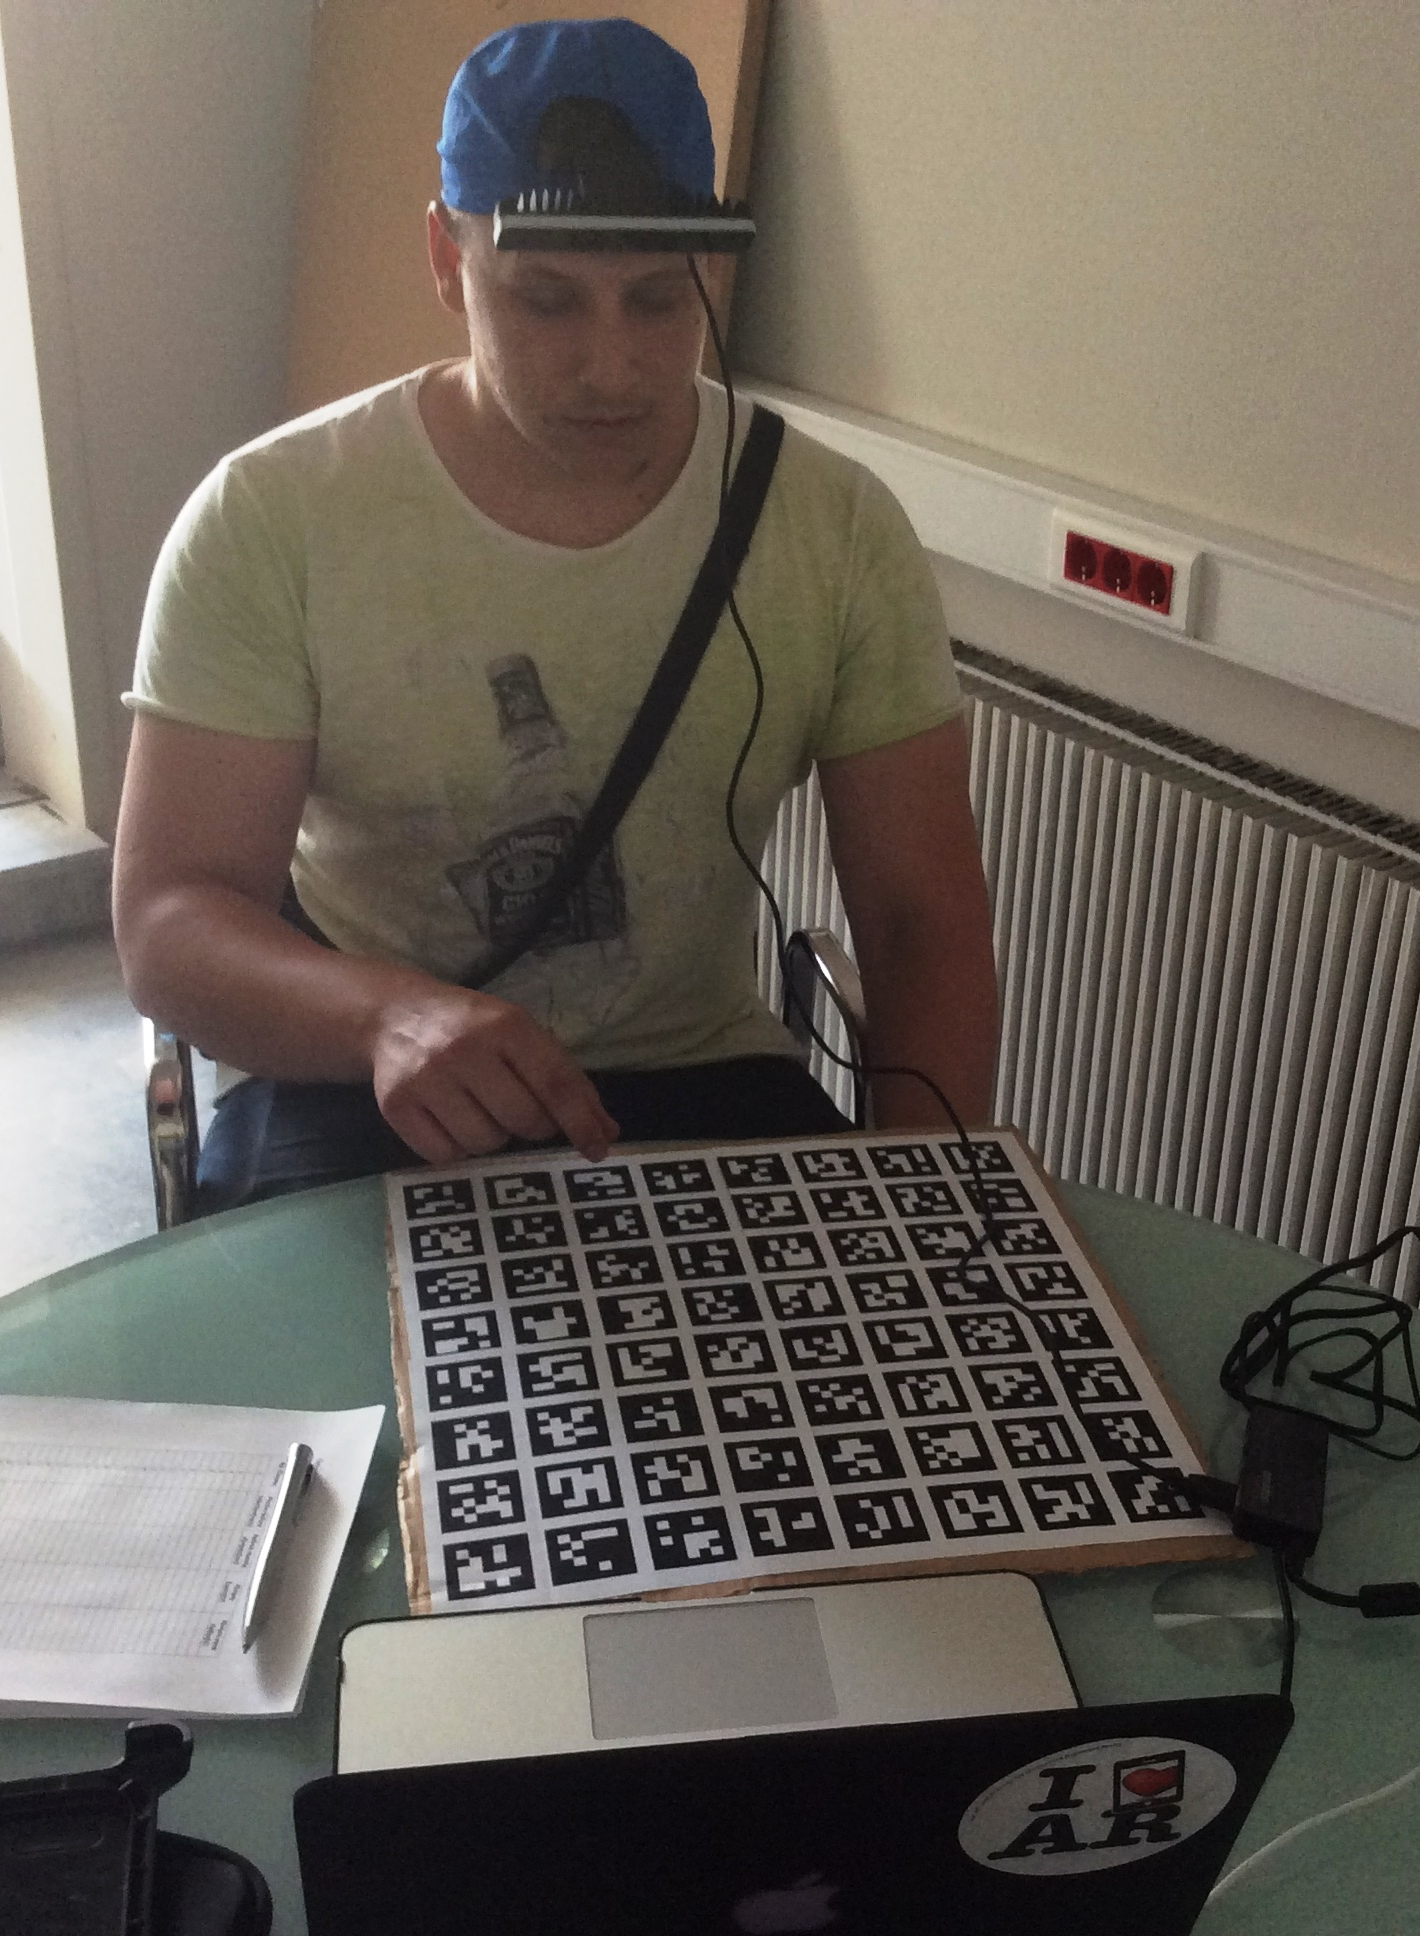
\includegraphics[width=.7\linewidth]{Files/Figures/user2.png}
  \caption{1b}
  \label{fig:sfig2}
\end{subfigure}\\
\caption{Φωτογραφία χρήστη κατά τη διάρκεια των δοκιμών}
\label{fig:test}
\end{figure}



\section{Διαδικασία Βαθμονόμησης}


Για την εύρεση των εσωτερικών παραμέτρων της κάμερας επιλέχθηκε η απλή, έτοιμη και αποτελεσματική λύση του εργαλείου βαθμονόμησης που παρέχεται μέσω της OpenCV. Η OpenCV διαθέτει έτοιμες συναρτήσεις και εργαλεία για την βαθμονόμηση της κάμερας που βασίζονται σε μεθόδους που αναφέρθηκαν στο κεφάλαιο 2. Επιπλέον μέσω της OpenCV μπορούμε να μάθουμε τους συντελεστές παραμόρφωσης της κάμερας. 


Για τη διεξαγωγή της βαθμονόμησης απαιτείται η χρήση μιας απλής, επίπεδης εικόνας ασπρόμαυρης σκακιέρας, που μπορεί να εκτυπωθεί με ένα κοινό εκτυπωτή. Η διαδικασία αυτή είναι αυτόματη, ενώ τα μόνα δεδομένα εισόδου που θα πρέπει να δώσουμε στο εργαλείο της OpenCV είναι ο αριθμός των εσωτερικών γωνιών των τετραγώνων της στις δύο κάθετες διευθύνσεις. Για παράδειγμα το πρότυπο της βαθμονόμησης φαίνεται στο σχήμα~\ref{fig:pattern}, όπου έχουμε μία σκακιέρα με αριθμό διαστάσεων με βάση τις εσωτερικές γωνίες 7x6.
Οι γωνίες τοποθετούνται σε σε ένα σύστημα 3D συντεταγμένων όπου z=0 (δηλαδή όλα τα σημεία βρίσκονται στο ίδιο επίπεδο). Η πληροφορία αυτή αξιοποιείται μέσω μεθόδων της OpenCV και επιστρέφονται ο πίνακας των εσωτερικών παραμέτρων της κάμερας και οι συντελεστές παραμόρφωσης. 



Η βαθμονόμηση της κάμερας πραγματοποιείται μόνο μία φορά σαν αρχικό βήμα (offline calibration) κατά το αρχικό στάδιο της ανάπτυξης της εφαρμογής. Πιο συγκεκριμένα, κάνουμε ξεχωριστό calibration για κάθε διαφορετικό μοντέλο κάμερας που μπορεί να χρησιμοποιηθεί στην αναπτυσσόμενη εφαρμογή, καθώς και για κάθε διαφορετική ανάλυση αυτών. Το αποτέλεσμα είναι ένα ξεχωριστό αρχείο για κάθε κάμερα και κάθε ανάλυση που περιέχει τις αντίστοιχες εσωτερικές παράμετρους. Ανάλογα με τον εξοπλισμό και τις επιλογές του χρήστη φορτώνεται κατά την έναρξη της εφαρμογής το ανάλογο αρχείο. Έτσι οι εσωτερικές παράμετροι είναι γνωστές, ώστε σε μεταγενέστερο στάδιο να βρεθούν οι εξωτερικές παράμετροι.



\begin{figure}[H]
    \centering
    \includegraphics[scale=0.6, angle=0]{Files/Figures/pattern.png}
    \caption[Πρότυπο σκακιέρας για τη βαθμονόμησης της κάμερας]{Πρότυπο σκακιέρας για τη βαθμονόμησης της κάμερας}
    \label{fig:pattern}
\end{figure}






Στο πλαίσιο της παρούσας εργασίας, έγινε βαθμονόμηση με λήψη εικόνων επίπεδης σκακιέρας με μέγεθος 7 x 6 εσωτερικών γωνιών, με χρήση του παραδείγματος της βιβλιοθήκης OpenCV. Το μέγεθος κάθε τετραγώνου της σκακιέρας ορίστηκε στα 2,5cm. Το πρότυπο αυτό καταγράφηκε μέσω της καμερας σε 25 διαφορετικές θέσεις. Η κάμερα διατηρήθηκε σε σταθερό σημείο και μετακινήσαμε την εκτυπωμένη εικόνα της σκακιέρας σε διαφορετικές θέσεις και με διαφορετικές κλίσεις. 



\begin{figure}
\begin{subfigure}{.5\textwidth}
  \centering
  \includegraphics[width=.9\linewidth]{Files/Figures/calibration.png}
  \caption{1a}
  \label{fig:calibration_screenshot1}
\end{subfigure}%
\begin{subfigure}{.5\textwidth}
  \centering
  \includegraphics[width=.9\linewidth]{Files/Figures/calib2.png}
  \caption{1b}
  \label{fig:calibration_screenshot2}
\end{subfigure}
\caption[Στιγμιότυπο κατά τη διαδικασία της βαθμονόμησης κάμερας μέσω της OpenCV]{Στιγμιότυπο κατά τη διαδικασία της βαθμονόμησης κάμερας μέσω της OpenCV}
\label{fig:calibration_screenshot}
\end{figure}


Η διαδικασία της βαθμονόμησης σε ανάλυση 640 x 480 έδωσε σαν αποτέλεσμα τις παρακάτω εσωτερικές παραμέτρους:


\begin{equation}
K=
\begin{bmatrix}
603.77848970443176 & 0 & 319.5\\
0 & 603.77848970443176 & 239.5\\
0 & 0 & 1
\end{bmatrix}
\end{equation}

Βλέποντας τις τιμές των principal points $c_{x}=319.5$ and $c{y}=239.5$ βλεπουμε ότι είναι περίπου στο κέντρο των επιλεγμένων διαστάσεων δηλαδή κοντά στις τιμές  320 (640/2) και 240(480/2). Επίσης βλέπουμε ότι $f_{x}=f_{y}$ που σημαίνει ότι χρησιμοποιείται κοινή εστιακή απόσταση και για τους 2 άξονες.


Εξ ορισμού η OpenCV μας δίνει 5 συντελεστές παραμόρφωσης, 3 ακτινικούς και 2 εφαπτομενικούς. Συγκεκριμένα κατά τη βαθμονόμηση πήραμε:

\begin{equation}
\begin{aligned}
k1= 0.16901284929874760\\
k2= -1.0214355567073656\\
p1= 0\\
p2= 0\\
k3= 1.3599972288823818 
\end{aligned}
\end{equation}

Το σφάλμα επαναπροβολής (Re-projection error) δίνει μία καλή εκτίμηση της ακρίβειας των παραμέτρων που βρέθηκαν κατά τη βαθμονόμηση της κάμερας. Η τιμή του πρέπει να είναι όσο γίνεται πιο κοντά στο 0. Υπολογίζεται με βάση τους πίνακες εσωτερικών παραμέτρων, συντελεστών παραμόρφωσης, περιστροφής και μετατόπισης. Πρέπει αρχικά να μετατρέψουμε το σημείο του αντικειμένου σε σημείο στην κάμερα. Έπειτα υπολογίζουμε την απόλυτη νόρμα ανάμεσα στο αποτέλεσμα που πήραμε με το μετασχηματισμό και με τον αλγόριθμο εύρεσης γωνιών. Για να βρούμε το μέσα σφάλμα υπολογίζουμε τον αριθμητικό μέσο των σφαλμάτων για όλες τις εικόνες βαθμονόμησης. Μετά τη διαδικασία βαθμονόμησης το σφάλμα που πήραμε ήταν πολύ κοντά στο 0 και συγκεκριμένα :

\begin{equation}
Avg_Reprojection_Error = 0.20315774320090751
\end{equation}


\section{Δημιουργία Markerboard}
%ΑΝΑΛΥΣΕ ΤΟ ARUCO FEATURE KAI ΠΩΣ ΓΙΝΕΤΑΙ ΤΟ MARKER TRACKING ΑΠΟ ΤΗΝ ARUCO ΚΑΙ ΤΟ BOARD.

Since the game of chess is a tabletop game that always uses a chessboard as a base for placing the chess pieces on, we considered that using a markerboard would be really similar to the use of a chessboard and the occlusion of the markerboard from the users hand would not affect the rendering of virtual chess pieces during a piece movement. That is why, we created a markerboard which consists of 64 markers in a 8x8 grid, just like a board that is used in chess games, as the main marker of the system. A paper published by the founders of ArUco described the methodology that can be used in order to create speci c marker IDs for the markerboard which will have a high number of bit transitions so that they are less likely to be confused with environment objects. While previous works impose xed dictionaries, the latest version of ArUco library proposes an automatic method for generating a board of marker with the desired number of markers and with the desired number of bits. We used the ArUco samples and created a board of highly reliable markers which corresponds to the size and dimensions of a real chessboard as described by the World Chess Organization.

\begin{figure}[H]
    \centering
    \includegraphics[scale=0.1, angle=0]{Files/Figures/markerboard.jpg}
    \caption[Το markerboard που δημιουργήθηκε μέσω της ArUco]{Το markerboard που δημιουργήθηκε μέσω της ArUco}
    \label{fig:ps3game}
\end{figure}

\section{Αναγνώριση Χειρονομίας Τσιμπήματος}
%ΠΩΣ ΑΚΡΙΒΩΣ ΚΑΝΩ ΤΗ ΧΕΙΡΟΝΟΜΙΑ ΤΣΙΜΠΗΜΑΤΟΣ-ΤΑ ΘΕΩΡΗΤΙΚΑ ΜΕΡΗ



Before describing the gestures that we implemented in our
system, we first discuss the challenges that we faced while
we designed our system and the high-level principles that we
followed to address them.

A small number of simple hand poses Although a human hand has 27 DOFs, only a few poses are comfortable and can be reproduced without training. Guided by this idea, we built our system mostly on the pinch pose inspired by Andrew Wilson’s [26] Thumb and Fore-Finger Interface. We use pinching as an analog of the mouse click to indicate the selection of an object. We also explore pointing for specifying remote locations, and touching the desktop with fingers to turn the desk surface into a multi-touch interface. 

-Use precise and memorable gestures 
To create precise and memorable gestures, we use metaphors that correspond closely to physical actions. We directly map 3D physical positions to virtual positions. Once a user understands a virtual scene, reaching for the object leverages his physical intuition to reach for a point in 3D space. We also adopt a physicallybasedmentalmodel to design hand gestures for rotation. Motivated by work showing that users tend to perform rotation and translation separately [15], we decouple camera rotation and camera translation as two distinct gestures to provide precise and physically-based control for both. 

-Limited hand motion 
Unrestricted 3D interactions and large movements are tiring and only useful for short periods of time. We exploit the desktop environment to address the fatigue issue and design our system such that users can rest their elbows or forearms on the desk most of the time. Inspired by the Eden system, [11], we also allow the user to pass objects between the hands (throw-and-catch) to minimize dragging. We also amplify the user’s 3D motion so that only small gestures are needed, e.g. we map a 10◦ hand rotation to 20◦ in the modeler.



Once the captured video frame has been stabilized and occlusion has been detected and defined in terms of binary blobs, the interaction problem becomes one of gesture recognition. As described in chapter 4, target occlusion is detected and defined relative to the target plane. Since all virtual augmentation is defined relative to the target plane, interaction between real and virtual objects can occur within this common coordinate system. One of the most significant contributions of this thesis is the following handbased interaction system using gesture recognition. Our goal is to provide a simple gesture recognition system for two-dimensional manipulative interaction. Currently, using a mouse to manipulate a window interface is commonplace. Our system provides a mouse-like gesture based interface to an immersed AR user without the need for the cumbersome mouse. To simulate a mouse requires the recognition of both point and select gestures in order to generate the appropriate mouse-down and mouse-up events at the indicated location. This goal is achieved without the need for a sophisticated gesture recognition system such as [OKA02] involving complex finger tracking for gesture inference through motion. Instead, the gesture model is specialized for the task of mouse replacement. Performing the gesture analysis in pattern-space simplifies the image processing and creates a very robust gesture recognition system.

In order to define the appropriate gestures, the requirements of the application must be defined in detail. The requirements of the gesture system discussed in this thesis are: • real-time performance • commercial pc and camera hardware • hand-based interaction without hardware or glove-based facilities The real-time requirement of the system poses great restriction on the level of gesture recognition that can be implemented. Commercial hardware may also limit system performance, as well as limit the quality of image capture on which all computer visionbased, image analysis techniques rely. The third requirement forces the use of computer vision to recognize hand gestures, which is performance bound by the processor. Given these restrictions an interactive application is described and a particular hand gesture model is defined. The goal of this interaction system is to provide the user with a virtual interface to control the augmentation system properties. In other words, the goal is to allow the user to change system parameters through gestures in real-time. The interface is designed to be a control panel that is augmented on the planar pattern. The user should be able to interact directly with this augmented control panel on the 2D planar pattern. This allows the user to directly manipulate the set of controls provided on the panel. The original 2D planar target pattern can be fixed in the environment or carried by the user and shown to the camera when the interaction is desired. For these reasons it is assumed that only one hand will be free to perform the gestures over the target pattern. With the application requirements described, a gesture model can be defined. Complex manipulation such as finger tapping can be recognized with the use of multiple cameras to capture finger depth information. However, under the constraints of a single camera system, the occlusion blob detection described in the previous chapter provides only two-dimensional information about the occluding hand. For this reason, the gesture language is based exclusively on hand posture. The hand is described in pixel-space as the union of the detected occlusion blobs (the occluder set found in chapter 4). Each blob representing a finger or a set of grouped fingers. Given that our goal is to replace a mouse, there are only two classifications to which the recognized hand postures can belong: a pointing posture and a selecting posture. The notion of pointing and selecting can vary between applications, so they must be clearly defined for each application. In this application, pointing is the act of indicating a location on the planar target relative to its top left corner. Selecting is the act of indicating the desire to perform an action with respect to the pointer location. In terms of the gesture model, the parameters associated with each posture are: a pointer location defined by the prominent finger tip and a finger count defined by the number of fingers detected by the system. With the gesture model defined, a gesture system can be constructed.

The gesture recognition system proposed in this chapter applies the defined gesture model to a working Augmented Reality application system. The system flow is shown in figure 5.1. The system begins by analyzing the captured video frame using computer vision techniques. At this point, posture analysis is performed to extract the posture parameters in order to classify the gesture. If classification succeeds, the recognized gesture is translated into the event-driven command understood by the interactive application.
%wang,popovi
Pinch / Click Detection A robust pinch detector is the basis
of our gestures, and we address it separately from 3D tracking.
Our pinch detection is based on detecting separation of
the tips of the index finger and thumb in at least one of the
two camera images. First, we check for extrema [18] of the
silhouette close to the predicted locations of the index finger
and thumb from our 3D pose estimate. Thumb-index separation
is detected if the geodesic distance between the extrema
is longer than the Euclidean distance. If no separation is detected
in either view, we register a pinch (Figure 12).

%--


The pinch is a basic gesture that can be used to interact on a 3D space rather than a pointing gesture that is usually used on 2D view systems, which is simpler and well performed. On a user-based gesture taxonomy developed [22], [30], several gestures such as ponting, pinch, grab, stretch (using both hands) have been classified according to user experience. The pinch gesture in an AR interaction space is performed several times to imply natural movements and other gestures like selection, shrink/stretch in different axis, rotation, either using one hand or both[30]. Hence, its recognition is fundamental for following basic interactions. On this work, we have implemented a pinch recognition algorithm that triggers a grabbing action to move and release virtual objects in the AR scene based on the hand coordinates exposed from the Leap Motion’s API. The algorithm, Figure 14 runs on a Hand Controller -explained in the next section- which gets the information tracked from the device. Once a hand is recognized, a list of fingers ordered from thumb[0] to pinky[4] are obtained. It consists on identify the thumb fingertip (thumb = finger[0]); calculate a fixed threshold value experimentally based on a proportion of 0.7 times the thumb’s size; from the Fingers list, obtain the fingertip position of each remaining fingers and compare the euclidean distance, equation 3.1 from the thumb to the current finger positions with the threshold value, if the resulting PinchDistance is lower, then a flag is activated, indicating that a pinch has been performed.Afterwards, the grabbing function is performed when the pinch flag is activated. It generates a bounding sphere around the pinch position of the thumb and initializes a vector GrabDistance that will be used to store the difference of distance from the pinch position to the found collided object -this is used to grab only a single object that is closer to the pinch position-; then it identifies each object that collides with the bounding sphere and updates the GrabDistance vector with the difference of the pinch position and the collided object. If the updated distance is less than the GrabDistance of the previous collided object, the object is set as grabbed and a force -a vector calculated from the difference of the pinch position and the position of the grabbed object- is added to the rigid body of the object in order to follow the position of the pinch. When the PinchDistance is higher, the grabbing and pinching flags are disabled. This grabbing function is based on [1] example algorithms.The design is compared with a built-in pinch strength measure from the SDK, the most recent version of the Leap Motion’s SDK provides an automatic measure of the pinch strength value that ranges from [0-1], where 0 corresponds to the open hand with fingers extended and 1 to a full pinch, varying while you move the thumb and other fingers toward each other. On the next chapter 4, the evaluation is explained in more detail



\section{Ανίχνευση Θέσης Τσιμπήματος}
%ΠΩΣ ΑΝΙΧΝΕΥΕΤΑΙ Η 3D ΘΕΣΗ ΤΣΙΜΠΗΜΑΤΟΣ ΜΕ ΒΑΣΗ ΤΗ ΜΕΘΟΔΟΛΟΓΙΑ ΜΟΥ


To determine the location of the user’s point and select actions, a pointer location must be chosen from the hand point set. To simplify this process, the current system constraints were exploited and a number of assumptions were made. The first useful constraint deals with the amount of target occlusion permitted. The planar tracking system used for augmentation assumes that approximately half of the target corners are visible at all times during the tracking phase. To satisfy this constraint, only a portion of a hand can occlude the target at any given time. For this reason, the assumption is made that the only portion of the hand to occlude the target will be the fingers. From this we get: Assumption 1: Separated fingers will be detected as separate blobs in the image analysis phase. Due to the simplicity of the desired interaction, a second assumption was made: Assumption 2: Fingers will remain extended and relatively parallel to each other.

The simple gesture model introduced in this chapter describes two gestures classified by the interaction system – point and selection. The point gesture is the combination of a single finger and a pointer location. A single group of fingers along with a pointer location is also classified as the gesture of pointing. The selection gesture is the combination of multiple fingers and a pointer location. Figure 5.3 shows an example of these two gestures, displayed in pattern-space. A sample point and select gesture are shown in figure 5.4(a) and 5.4(b) respectively. These images are the grayscale representations of full colour screenshots. In this demonstration application the gesture system recognizes the colour region occupied by the finger pointer and also recognizes when selection has occurred. The fact that selection has been recognized from the two finger blobs is shown clearly in the text annotation at the top of the figure.

The interaction created by this gesture model is a point and select mechanism similar to the commonly used mouse interaction with a window-based operating system. To allow a closed system of human-computer interaction, the actions generated by the hand gestures define a set of system states. The possible states of the gesture system are pointing, selecting and no hand detection. The transitions between states are triggered by a change in finger count. This transition is represented by a pair of values, (cp,cc), indicating the previous and current finger counts. The possible values for cp and cc are 0, indicating no hand detection, 1, indicating a single detected finger pointer, and n, indicating more than one detected finger pointer. This state machine is shown in figure 5.5 and the system begins in the no hand detection state.


\begin{figure}
\begin{subfigure}{.5\textwidth}
  \centering
  \includegraphics[width=.8\linewidth]{Files/Figures/2.png}
  \caption{1a}
  \label{fig:sfig1}
\end{subfigure}%
\begin{subfigure}{.5\textwidth}
  \centering
  \includegraphics[width=.8\linewidth]{Files/Figures/3.png}
  \caption{1b}
  \label{fig:sfig2}
\end{subfigure}\\
\begin{subfigure}{.5\textwidth}
  \centering
  \includegraphics[width=.8\linewidth]{Files/Figures/4.png}
  \caption{1a}
  \label{fig:sfig1}
\end{subfigure}%
\begin{subfigure}{.5\textwidth}
  \centering
  \includegraphics[width=.8\linewidth]{Files/Figures/5.png}
  \caption{1b}
  \label{fig:sfig2}
\end{subfigure}
\caption{Pinch Gesture Detection Phases}
\label{fig:fig}
\end{figure}




\section{Tαυτοποίηση Συστημάτων Συντεταγμένων}

Coordinate Systems Matching A first step is to consider a unified coordinate system between the AR target and hand tracking sensor. The simplest coordinate systems matching is based on the assumption that our AR marker and sensor are placed on the same origin, when this is not the case, i.e. the sensor and marker are placed in different areas from the camera view perspective, a translation of the Leap Motion’s pose matrix needs to be performed by using the AR marker as a reference. A solution to this, is to use the image target to act as the world center and bring the Leap Motion’s coordinate system by multiplying the inverse pose of our main target (image target) by the pose of the Leap Motion’s target. This creates an offset matrix that can be used to bring points from Leap Motion to image target coordinate system[47]. Nevertheless, for our prototype purpose, it is assumed that the AR marker and sensor are placed in the same origin, where it matches both coordinate systems. This is done, both programmatically, through the game engine and physically where are adjusted in the same origin from a camera view perspective as seen on the Figure.


\section{Απεικόνιση Εικονικών Αντικειμένων} \label{s:rendering}
%clarke


As last part of the experimental studies 3D objects are rendered onto the views. the virtual camera uses the pose calculated by the ArUco's algorithm which should be placed at the same position as the real camera. 

Using the calculated camera poses virtual objects have been rendered onto the images. Knowing where the object should be placed in the real world is essential for an augmented reality application. 



%σελ 25 jimenez
Although the Unity platform deals with the graphics and integration of libraries for this project, it is necessary to give a deeper review of the process by explaining the target pose calculation and content positioning in the AR framework and the hand controller’s integration. The AR framework exposes a 3x4 Pose Matrix, equation 3.2 that represents the pose of a target with respect to the camera plane. The left 3X3 matrix expresses the rotation matrix, which indicates how the target is rotated while the right column is the translation vector, which is the position of the target as seen from the camera[47], e.g. an identity matrix indicates that the target is parallel to the camera plane (rotation) and a vector (0,0,0) indicates the camera and the target are in the same position.

To position content on the target, the first step is to know the projection matrix -4x4 matrix that projects the scene to the image plane of the camera[49]- that is created with the intrinsic camera calibration parameters, vuforia uses a right handed coordinate system (with the camera origin pointing into the positive z-axis, x-axis to the right and y-axis is downwards) because it is the same coordinate system for targets (just rotated 90 degrees around the x axis: x-axis to the right, y-axis is upwards and z-axis points out of the target-plane; in Unity, z-axis is upwards and y-axis points out of the target)[47]. Once we know the projection matrix we need to set a perspective frustrum from it, where a near and far planes must be set and the size of our trackable -defined in the dataset with feature- should fall within these two planes, Figure 18.
With these requirements in mind, the virtual content (vertices, normals, indices, texture coordinates)
is placed according to the pose matrix calculated at runtime.
The Leap Motion coordinates can be used to move a virtual object, firstly, normalizing and
transforming to suitable coordinates in the interaction box, Figure 13 explained previously.

\section{Χειρισμός Εικονικών Αντικειμένων} \label{s:manipulation}
%ΠΩΣ ΜΕΤΑΚΙΝΟΥΝΤΑΙ ΤΑ ΠΙΟΝΙΑ ΜΕ ΒΑΣΗ ΤΟΝ ΑΛΓΟΡΙΘΜΟ ΜΟΥ
%wang-paris-popovi

-Object translation 
When the user pinches with one hand,
we select the closest object, and translate according to the
pinching hand.


%mcdonald
With this visual feedback mechanism in place, a mechanism for initiating interaction with the controls on the panel is needed. The behaviour associated with control manipulation is defined in the normal event driven, object-oriented fashion associated with window– based application programming. Applying the gesture model to this augmented interaction requires only a simple communicative translation between the gestures, including posture parameters, and the event-based control manipulation. This translation is defined in terms of the gesture state machine outlined in figure 5.5. For example, when a selection gesture is recognized immediately following a pointing gesture, a mouse-down event is sent to the actual control panel dialog, along with the pointer location parameter as if it were sent by the mouse hardware. This way, when the gesture occurs over a button on the virtual panel, the event generates the equivalent button press on the dialog box. On the other hand, when a pointing gesture immediately follows a selection gesture, a mouse-up event is sent


\section{Αντιμετώπιση Απόκρυψης Αντικειμένων} \label{s:occlusion}
%OCCLUSION HANDLING

In this section, the depth estimation of real world is described.
The depth estimation is used to compose the image
of the virtual objects and the image of the real world without
occlusion conflicts. In order to avoid occlusion conflicts, we
need the depth information of only the region onto which
virtual objects are projected. When the positions of virtual
objects are known, the region for depth estimation can be
limited as shown in Figure 4. Therefore, the depth estimation
region of real world can be determined by projecting
a CG object’s bounding box using the model-view matrix
estimated in Section 3.1. The following steps describe a
method of depth estimation of real world.
1. A position of the CG object in the world coordinate
system is transformed into its position in the camera
coordinate system using the estimated model-view matrix
M.
2. A bounding box of the virtual object is projected onto
the left image as shown in Figure 4. A depth estimation
region is obtained as a bounding rectangle of the
projected box. The same process is done for the right
image as well.
3. By adopting the Sobel filter, edges are detected in the
region of depth estimation on the left and right images
4. Stereo matching is performed and the depth value is
computed. Note that only pixels on detected edges in
the left image are matched to those in the right image,
matching window size is 5 x 5 pixels, and similarity
measure is the sum of absolute differences (SAD). In
the same way, the right image as a reference image is
matched to the left image.
5. Matching errors are excluded by considering the consistency
between left-to-right and right-to-left matchings.
The depth values at the pixels between the edges
are interpolated.

By using the estimated model-view matrix and the depth
map of the real world, CG images of virtual objects are
mixed into the image of real world. At this stage, the depth
of real world and each virtual object are compared. When
the real objects are closer to the user’s viewpoint, a transparent
virtual object is drawn at the 3-D position where the
real objects exist. By using a hardware z buffering algorithm,
the virtual objects that are farther than the transparent
objects are not actually drawn on the frame buffer. Therefore
the composed image is looked as if the real objects are
occluding the virtual objects. These rendering steps are illustrated
with examples in Figure 5.
First, only the background image of a real scene is rendered
on the frame buffer as in Figure 5 (a). Z-buffer value
is also set to the farthest value through out the screen. Then,
Z-buffer of the real objects are set to the depth of the real
objects in Figure 5 (c). The regions of real objects are illustrated
with gray levels of depth in Figure 5 (b). Finally, the
virtual objects are rendered by using the model-view matrix
in Figure 5 (d),(e). These steps are applied to both left and right images for obtaining a stereo pair of composite
images.

%-----
Για να μπορέσει ένας χρήστης να εκτελέσει επιτυχώς ορισμένες διεργασίες σε περιβάλλοντα επαυξημένης πραγματικότητας, χρειάζεται να παρέχεται από το σύστημα ένα συγκεκριμένο επίπεδο "εμβύθισης" του χρήστη. Πρέπει δηλαδή ο χρήστης να πιστέψει, όσο γίνεται, ότι τα εικονικά αντικείμενα είναι πραγματικά. 
Στις περισσότερες προσεγγίσεις, οι αποκρύψεις των εικονικών αντικειμένων δεν λαμβάνονται υπ'όψην και επομένως τα εικονικά αντικείμενα απεικονίζονται πάντα πάνω από το frame του βίντεο, συνεπώς πάνω από τα πραγματικά αντικείμενα της σκηνής. 
Ωστόσο, για να δημιουργηθούν καθηλωτικές και ρεαλιστικές εφαρμογές, η απόκρυψη ανάμεσα στα εικονικά και τα πραγματικά αντικείμενα πρέπει να πραγματοποιηθεί σωστά, ώστε οι χρήστες να μπορούν να κοιτάξουν σε μία σκηνή, όπου το εικονικό περιεχόμενο θα είναι εναρμονισμένο με το φυσικό περιβάλλον. Μία τέτοια προσέγγιση μας επιτρέπει να πετύχουμε υψηλό επίπεδο "εμβύθισης" αφού τα εικονικά αντικείμενα μπορούν να εναρμονιστούν με τα χέρια του χρήστη, ώστε να εμφανίζεται σωστά το ένα πάνω από το άλλο ή το αντίθετο. 

Κάτι τέτοιο συνήθως δε συμβαίνει στις περισσότερες εφαρμογές επαυξημένης πραγματικότητας. Στην OpenGL, όταν ένα αντικείμενο απεικονίζεται στην οθόνη, το βάθος ενός pixel που παράγεται (z coordinate) αποθηκεύεται σε ένα buffer που ονομάζεται z-buffer ή buffer βάθους (depth buffer). Αυτός ο buffer ορίζεται συνήθως ως ένα δισδιάστατος πίνακας (x-y) με ένα στοιχείο για κάθε εικονοστοιχείο της οθόνης. Αν κάποιο άλλο αντικείμενο της σκηνής πρέπει να απεικονιστεί στο ίδιο εικονοστοιχείο, η μέθοδος συγκρίνει τα 2 βάθη και αντικαθιστά το τρέχων εικονοστοιχείο, αν το αντικείμενο είναι πιο κοντά στο θεατή. Έπειτα, το επιλεγμένο βάθος αποθηκεύεται στο z-buffer, αντικαθιστώντας την προηγούμενη τιμή. Εν τέλει, ο z-buffer θα επιτρέψει στη μέθοδο να αναπαράγει σωστά την αντίληψη του βάθους, δηλαδή το γεγονός ότι ένα αντικείμενο που βρίσκεται πιο κοντά θα πρέπει να κρύβει ένα άλλο που βρίσκεται πιο μακριά.


Το κύριο πρόβλημα που εμφανίζεται προκειμένου και εμποδίζει την αντιμετώπιση του φαινομένου της απόκρυψης στα επαυξημένα περιβάλλοντα βρίσκεται στο γεγονός ότι, συνήθως, δεν υπάρχει πληροφορία για το βάθος της σκηνής. Για να ξεπεραστεί αυτό το πρόβλημα, πρέπει να αξιοποιηθεί το βάθος της πραγματικής σκηνής όπως το βλέπει ο χρήστης, δηλαδή ως προς τη θέση του χρήστη. 

Στην παρούσα διπλωματική εργασία, χρησιμοποιήθηκε ο αισθητήρας βάθους της κάμερας Realsense 3D, για την υποστήριξη της διαδικασίας απόκτησης ενός χάρτη βάθους της σκηνής του περιβάλλοντος. O αισθητήρας αυτός μπορεί να μετρήσει την απόσταση κάθε αντικειμένου που βλέπει, δημιουργώντας ένα χάρτη βάθους. Με αυτό τον τρόπο το βάθος κάθε pixel του depth frame μπορεί να εκτιμηθεί. Η εικόνα βάθους είναι ουσιαστικά ένας πίνακας διαστάσεων 640 x 480  όπου η τιμή κάθε pixel αναπαριστά την απόσταση της κάμερας βάθους από το συγκεκριμένο σημείο στο 3D χώρο (σε χιλιοστά). 


Όταν μία κάρτα βίντεο απεικονίζει μία εικονική σκηνή, υπολογίζει την απόκρυψη μέσω του depth buffer, δηλαδή την απόσταση z κάθε αντικειμένου από την εικονική σκηνή. Συνήθως, όταν ένα άλλο εικονικό αντικείμενο πρέπει να απεικονιστεί στο ίδιο pixel του z-buffer, η μέθοδος συγκρίνει τα 2 βάθη και αντικαθιστά το τρέχων pixel αν το αντικείμενο είναι πιο κοντά στον παρατηρητή, δηλαδή την κάμερα.

Το τέχνασμα που χρησιμοποιείται είναι η αρχικοποίηση του Z-Buffer της OpenGL με τις τιμές βάθους που παίρνουμε από τον αισθητήρα πριν την απεικόνιση ενός 3D εικονικού αντικειμένου και αφού απεικονίσουμε το πολύγωνο που δείχνει την έγχρωμη εικόνα που καταγράφει το βίντεο. Με αυτό τον τρόπο, όταν τα εικονικά πιόνια απεικονίζονται στην οθόνη, θα αποκρύπτονται από τα χέρια του χρήστη ή από οποιοδήποτε άλλο αντικείμενο περάσει από πάνω τους. 

Η διαδικασία αυτή μοιάζει με την προσομοίωση της απεικόνισης ενός ολόκληρου περιβάλλοντος 3D και τη χρήση των τιμών του z-buffer. Eπομένως, προκειμένου να αντιμετωπίσουμε το πρόβλημα της απόκρυψης αντικειμένων (occlusion handling) έπρεπε να αντιστοιχήσουμε ολόκληρη το χάρτη βάθους στην έγχρωμη εικόνα που καταγράφεται, να μετατρέχουμε τις τιμές βάθους από χιλιοστά σε μέτρα και μετά να γράψουμε κάθε τιμή στο z-buffer της OpenGL.


Ώστόσο, πριν φτάσουμε στο σημείο να γράψουμε στο z-buffer, πρέπει να λάβουμε υπ'οψην μας το είδος της προβολής που χρησιμοποιείται από την OpenGL στην εφαρμογή μας (ορθή ή προοπτική). 


Στη συγκεκριμένη περίπτωση, το είδος της προβολής με την οποία απεικονίζονται τα εικονικά αντικείμενα της σκηνής είναι η προοπτική προβολή και πρέπει να τροποποιήσουμε τα δεδομένα με βάση αυτή. Σε αυτό το είδος προβολής, η σχέση ανάμεσα στην τιμή Z και το βάθος είναι μη-γραμμική και συγκεκριμένα της μορφής:



\begin{equation}
\begin{aligned}
depth=\frac{A}{Z}+B \\
A=\frac{Z_{far}Z_{near}}{Z_{far}-Z_{near}}\\ B=\frac{Z_{far}}{Z_{far}-Z_{near}}
\end{aligned}
\end{equation}

Τέλος πρέπει να προσέξουμε το γεγονός ότι τα σημεία μπροστά από το σημείο παρατήρησης (viewpoint) στην OpenGL έχουν αρνητικές τιμές συντεταγμένων στον άξονα Z. Αφού εφαρμόσουμε το μετασχηματισμό που αναφέρθηκε με την προηγούμενη εξίσωση, μπορούμε να γράψουμε τις τιμές των δεδομένων στον z-buffer. Μόλις συμβεί αυτό, παρατηρούμε ότι τα πραγματικά και τα εικονικά αντικείμενα "δένουν" αρμονικά μαζί στη σκηνή με αρκετά μεγάλη ακρίβεια. 




\section{Ενσωμάτωση Μηχανής Σκακιού}

Μετά την υλοποίηση του αλγορίθμου ανίχνευσης της χειρονομίας του "τσιμπήματος" και την αντιμετώπιση του προβλήματος απόκρυψης αντικειμένων, κρίθηκε απαραίτητο, ο χρήστης να μπορεί να παίξει ένα παιχνίδι σκακιού ενάντια στον υπολογιστή. Με αυτό τον τρόπο, πετχαίνουμε μία φυσική αλληλουχία γεγονότων στο παιχνίδι του σκακιού και προσμοιώνουμε ολοκληρωμένα ένα πραγματικό παιχνίδι σκακιού απέναντι σε έναν αντίπαλο, κάτι που θα μας βοηθήσει στη συνέχεια με την αξιολόγηση του συστήματος. 


Για να μπορέσει ο χρήστης να παίξει σκάκι ενάντια στον υπολογιστή, κανονικά θα έπρεπε να υλοποιηθούν αλγόριθμοι τεχνητής νοημοσύνης που θα επέτρεπαν στο πρόγραμμα μας να καθορίσει την επόμενη κίνηση του υπολογιστή με βάση τις προηγούμενες κινήσεις που έλαβαν μέρος κατά τη διάρκεια του παιχνιδιού. Ωστόσο η υλοποίηση τέτοιων αλγορίθμων για την εφαρμογή μας δεν βρίσκεται μέσα στους σκοπούς της παρούσας διπλωματικής εργασίας και έπρεπε να αναζητηθεί ένα απλός τρόπος για την ενσωμάτωση λειτουργιών τεχνητής νοημοσύνης. 


Εκεί ακριβώς προκύπτει η λύση των μηχανών σκακιού. Μία μηχανή σκακιού δεν είναι τίποτα άλλο από ένα πρόγραμμα υπολογιστή το οποίο δέχεται σαν είσοδο την θέση ενός πιονιού στη σκακιέρα, αναλύει τις θέσεις όλων των πιονιών και υπολογίζει την καλύτερη δυνατή κίνηση με βάση τη διάταξη των πιονιών στη σκακιέρα μέσα σε ένα χρονικό περιθώριο που ορίζεται εκ των προτέρων. Η μηχανή σκακιού μπορεί να εκτιμήσει τις επόμενες κινήσεις, αλλά συνήθως δεν αλληλεπιδρά απευθείας με το χρήστη, καθώς οι περισσότερες μηχανές δεν έχουν δική του γραφική διεπαφή για την επικοινωνία με το χρήστη. Αντίθετα οι περισσότερες είναι εφαρμογές κονσόλας που επικοινωνούν με μία γραφική διεπαφή μέσω ενός καθορισμένου πρωτοκόλλου. Αυτό επιτρέπει στο χρήστη να παίζει ενάντια σε πολλές διαφορετικές μηχανές χωρίς να χρειάζεται να εκπαιδευτεί εκ νέου σε νέες διεπαφές κάθε φορά και επιτρέπει σε διαφορετικές μηχανές να παίζουν η μία ενάντια στην άλλη. Στη συγκεκριμένη περίπτωση, η εφαρμογή μας παίζει το ρόλο της γραφικής διεπαφής ως τώρα. 


Στις μέρες μας, ο πιο πιο γνωστός τρόπος επικοινωνίας με μηχανές σκακιού πραγματοποιείται μέσω ενός πρωτοκόλλου που ονομάζεται Universal Chess Interface (UCI) Protocol. Πρόκειται για ένα πρωτόκολλο ανοιχτής επικοινωνίας που επιτρέπει σε μία μηχανή σκακιού ενός προγράμματος να επικοινωνεί με τη διεπαφή χρήστη μέσα από ένα σύνολο αυστηρά καθορισμένων εντολών. Επομένως, για να ενσωματώσουμε μία μηχανή σκακιού στην εφαρμογή μας, πρέπει να βρούμε ένα τρόπο ώστε να γίνει ανταλλαγή εντολών (συμβολοσειρές) ανάμεσα στην εφαρμογή μας και τη μηχανή σκακιού. 


Η μηχανή δέχεται εντολές μέσω standard input από μια εφαρμογή και παράγει τις απαντήσεις σε συμβολοσειρές του standard output. Δεν έχει δηλαδή γραφική διεπαφή, είσοδο μέσω ποντικιού ή εικόνες, παρά μόνο ένα απλό παράθυρο κονσόλας, που δεν είναι τίποτα περισσότερο παρά ένα εκτελέσιμο (.exe) αρχείο. Προκειμένου να υλοποιηθεί αυτή η επικοινωνία με το εκτελέσιμο αρχείο μιας μηχανής σκακιού αποφασίστηκε να αξιοποιηθεί η δυνατότητα που προσφέρει η βιβλιοθήκη Qt μέσω μιας κλάσης με το όνομα QProcess, η οποία επιτρέπει στο πρόγραμμά μας να εκκινήσει ένα εκτελέσιμο αρχείο, καθώς και να διαβάσει και να γράψει εντολές συμβολοσειρών από και προς αυτό. Η αλληλεπίδραση με τη μηχανή σκακιού ξεκινά με μία εντολή "uci", η οποία επικοινωνεί με τη μηχανή λέγοντας της να ταυτοποιήσει τον εαυτό της, δηλαδή να δώσει σαν έξοδο τα χαρακτηριστικά της όπως την ονομασία της, την έκδοσή της κλπ.  Έπειτα, δέχεται εντολές που μπορούν να αλλάξουν ορισμένες προεπιλεγμένες τιμές ιδιοτήτων που επηρεάζουν τα δεδομένα τα οποία θα προβάλλονται σαν έξοδος από τη μηχανή. Μετέπειτα, η μηχανή δέχεται ως είσοδο από την εφαρμογή μας την κίνηση που πραγματοποίησε ο χρήστης και εξάγει την επόμενη καλύτερη κίνηση που μπορεί να εκτελέσει ο αντίπαλος, δηλαδή ο υπολογιστής.
Η μηχανή σκακιού δέχεται σαν παράμετρο το χρόνο τον οποίο έχει για να υπολογίσει την κίνηση αυτή, ψάχνοντας για την καλύτερη δυνατή κίνηση. Ξεκινά την αναζήτηση και εκτιμά την καλύτερη κίνηση που υπάρχει πριν λήξει το χρονικό περιθώριο που ορίζεται στην αρχή της εκτέλεσης της μηχανής. 

Για την εφαρμογή μας, θεωρήσαμε ότι το χρονικό αυτό περιθώριο πρέπει να είναι ιδιαίτερα μικρό (40ms), ώστε να μην "παγώνει" η απεικόνιση των εικονικών αντικειμένων και να μπορούμε να παίρνουμε άμεσα feedback από το πρόγραμμα. Συνήθως οι μηχανές σκακιού δεν έχουν τη δυνατότητα να αντιλαμβάνονται αν μία εντολή κίνησης που δίνεται από το χρήστη είναι έγκυρη ή όχι, με βάση τον τύπο των πιονιών και την κατάσταση της σκακιέρας. Για το λόγο αυτό επιλέχθηκε να χρησιμοποιηθεί η μηχανή iCE [link], η οποία ελέγχει αν η κίνηση που γίνεται είναι επιτρεπτή ή όχι. Αν η κίνηση δεν επιτρέπεται, τότε η μηχανή επιστρέφει ως έξοδο τη συμβολοσειρά "Invalid chess move". Αυτή η ιδιότητα επιτρέπει την υλοποίηση μιας αρχιτεκτονικής στον κώδικά μας, η οποία δε θα είναι επιρρεπής σε λανθασμένες κινήσεις όταν αυτές γίνονται κατά λάθος από το χρήστη. Επιπλέον, η μηχανή που χρησιμοποιήθηκε μπορεί να ανιχνεύσει αν το παιχνίδι ολοκληρώθηκε και ποιος είναι νικητής ώστε να μπορούμε να ενημερώσουμε το χρήστη για το αποτέλεσμα του παιχνιδιού. 

Συμπερασματικά, υλοποίησαμε τη βασική λειτουργικότητα για την αποστολή και λήψη συμβολοσειρών προς και από τη μηχανή σκακιού και με βάση αυτές τις συμβολοσειρές το πρόγραμμά μας εκτελεί συγκεκριμένες δράσεις.










